\section{Undetermined Coefficients for Higher Order Equations}

\noindent
In this section we consider the constant coefficient equation
\begin{equation}
  \label{eq:9.3.1}a_{0}y^{(n)}+a_{1}y^{(n-1)}+\cdots+a_{n}y=F(x),
\end{equation}
where $n\ge3$ and $F$ is a linear combination of functions of the form
\[
  e^{\alpha x}\left(p_{0}+p_{1}x+\cdots+p_{k}x^{k}\right)
\]
or
\[
  e^{\lambda x}\left[\left(p_{0}+p_{1}x+\cdots+p_{k}x^{k}\right) \cos\omega x+ \left(q_{0}+q_{1}x+\cdots+q_{k}x^{k}\right) \sin\omega x\right].
\]

From Theorem~9.1.5, the general solution of \eqref{eq:9.3.1} is $y=y_{p}+y_{c}$, where $y_{p}$ is a
particular solution of \eqref{eq:9.3.1} and $y_{c}$ is the general solution of the complementary
equation
\[
  a_{0}y^{(n)}+a_{1}y^{(n-1)}+\cdots+a_{n}y=0.
\]
In Section~9.2 we learned how to find $y_{c}$. Here we will learn how to find $y_{p}$ when the
forcing function has the form stated above. The procedure that we use is a generalization of the
method that we used in Sections~5.4 and 5.5, and is again called {\color{blue}\it method of
undetermined coefficients\/}. Since the underlying ideas are the same as those in Sections~5.4 and
5.5, we'll give an informal presentation based on examples.

\boxit{Forcing Functions of the Form $e^{\alpha x}\left(p_{0}+p_{1}x+\cdots+p_{k}x^{k}\right)$}

\noindent
We first consider equations of the form
\[
  a_{0}y^{(n)}+a_{1}y^{(n-1)}+\cdots+a_{n}y=e^{\alpha x}\left(p_{0}+p_{1}x+\cdots+p_{k}x^{k}\right).
\]

\begin{example}
  \label{example:9.3.1} \rm Find a particular solution of
  \begin{equation}
    \label{eq:9.3.2}y'''+3y''+2y'-y=e^{x}(21+24x+28x^{2}+5x^{3}).
  \end{equation}
\end{example}

\solution Substituting
\begin{eqnarray*}
  y    & = & ue^{x},           \\
  y'   & = & e^{x}(u'+u),      \\
  y''  & = & e^{x}(u''+2u'+u), \\
  y''' & = & e^{x}(u'''+3u''+3u'+u)
\end{eqnarray*}
into \eqref{eq:9.3.2} and canceling $e^{x}$ yields
\[
  (u'''+3u''+3u'+u)+3(u''+2u'+u)+2(u'+u)-u =21+24x+28x^{2}+5x^{3},
\]
or
\begin{equation}
  \label{eq:9.3.3}u'''+6u''+11u'+5u=21+24x+28x^{2}+5x^{3}.
\end{equation}
Since the unknown $u$ appears on the left, we can see that \eqref{eq:9.3.3} has a particular
solution of the form
\[
  u_{p}=A+Bx+Cx^{2}+Dx^{3}.
\]
Then
\begin{eqnarray*}
  u_{p}'   & = & B+2Cx+3Dx^{2} \\
  u_{p}''  & = & 2C+6Dx        \\
  u_{p}''' & = & 6D.
\end{eqnarray*}
Substituting from the last four equations into the left side of \eqref{eq:9.3.3} yields
\begin{eqnarray*}
  u_{p}'''+6u_{p}''+11u_{p}'+5u_{p} & = & 6D+6(2C+6Dx)+11(B+2Cx+3Dx^{2}) \\
                                    &   & +5(A+Bx+Cx^{2}+Dx^{3})         \\
                                    & = & (5A+11B+12C+6D)+(5B+22C+36D)x  \\
                                    &   & +(5C+33D)x^{2}+5Dx^{3}.
\end{eqnarray*}
Comparing coefficients of like powers of $x$ on the right sides of this equation and
\eqref{eq:9.3.3} shows that $u_{p}$ satisfies \eqref{eq:9.3.3} if
\[
  \begin{array}{rcr}
    5D                       & = & 5\phantom{.}  \\
    5C+33D                   & = & 28\phantom{.} \\
    5B+22C+36D               & = & 24\phantom{.} \\
    5A+11B+12C+\phantom{3}6D & = & 21.
  \end{array}
\]
Solving these equations successively yields $D=1$, $C=-1$, $B=2$, $A=1$. Therefore
\[
  u_{p}=1+2x-x^{2}+x^{3}
\]
is a particular solution of \eqref{eq:9.3.3}, so
\[
  y_{p}=e^{x}u_{p}=e^{x}(1+2x-x^{2}+x^{3})
\]
is a particular solution of \eqref{eq:9.3.2} (Figure~\ref{figure:9.3.1}).

\begin{figure}[tbp]
  \centering
  \color{blue}
  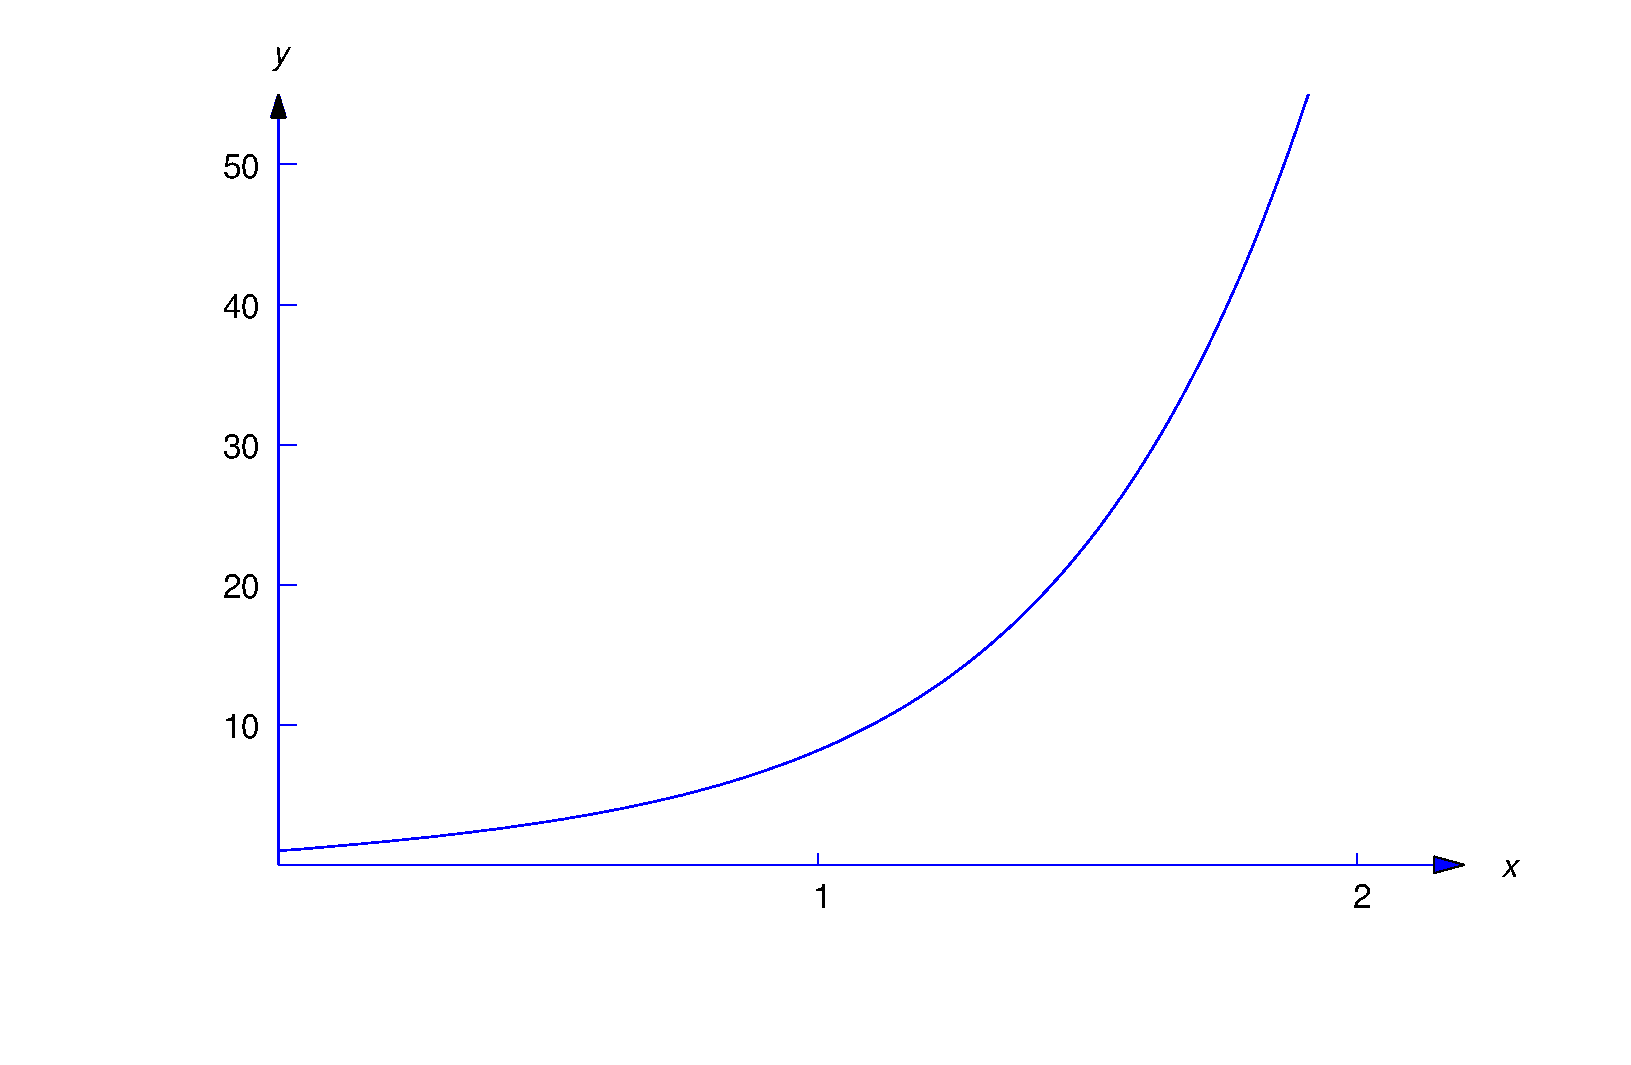
\includegraphics[bb=-78 148 689 643, width=5.67in, height=3.66in, keepaspectratio]{fig090301}
  \caption{$y_{p}=e^{x}(1+2x-x^{2}+x^{3})$ }
  \label{figure:9.3.1}
\end{figure}

\begin{example}
  \label{example:9.3.2} \rm Find a particular solution of
  \begin{equation}
    \label{eq:9.3.4}y^{(4)}-y'''-6y''+4y'+8y=e^{2x}(4+19x+6x^{2}).
  \end{equation}
\end{example}

\solution Substituting
\begin{eqnarray*}
  y       & = & ue^{2x},                   \\
  y'      & = & e^{2x}(u'+2u),             \\
  y''     & = & e^{2x}(u''+4u'+4u),        \\
  y'''    & = & e^{2x}(u'''+6u''+12u'+8u), \\
  y^{(4)} & = & e^{2x}(u^{(4)}+8u'''+24u''+32u'+16u)
\end{eqnarray*}
into \eqref{eq:9.3.4} and canceling $e^{2x}$ yields
\begin{eqnarray*}
   &  & (u^{(4)}+8u'''+24u''+32u'+16u)-(u'''+6u''+12u'+8u) \\
   &  & -6(u''+4u'+4u)+4(u'+2u)+8u=4+19x+6x^{2},
\end{eqnarray*}
or
\begin{equation}
  \label{eq:9.3.5}u^{(4)}+7u'''+12u''=4+19x+6x^{2}.
\end{equation}
Since neither $u$ nor $u'$ appear on the left, we can see that \eqref{eq:9.3.5} has a particular
solution of the form
\begin{equation}
  \label{eq:9.3.6}u_{p}=Ax^{2}+Bx^{3}+Cx^{4}.
\end{equation}
Then
\begin{eqnarray*}
  u_{p}'      & = & 2Ax+3Bx^{2}+4Cx^{3} \\
  u_{p}''     & = & 2A+6Bx+12Cx^{2}     \\
  u_{p}'''    & = & 6B+24Cx             \\
  u_{p}^{(4)} & = & 24C.
\end{eqnarray*}
Substituting $u_{p}''$, $u_{p}'''$, and $u_{p}^{(4)}$ into the left side of \eqref{eq:9.3.5} yields
\begin{eqnarray*}
  u_{p}^{(4)}+7u_{p}'''+12u_{p}'' & = & 24C+7(6B+24Cx)+12(2A+6Bx+12Cx^{2}) \\
                                  & = & (24A+42B+24C)+(72B+168C)x+144Cx^{2}.
\end{eqnarray*}
Comparing coefficients of like powers of $x$ on the right sides of this equation and
\eqref{eq:9.3.5} shows that $u_{p}$ satisfies \eqref{eq:9.3.5} if
\[
  \begin{array}{rcr}
    144C                   & = & 6\phantom{.}  \\
    72B+168C               & = & 19\phantom{.} \\
    24A+42B+\phantom{1}24C & = & 4.
  \end{array}
\]
Solving these equations successively yields $C=1/24$, $B=1/6$, $A=-1/6$. Substituting these into
\eqref{eq:9.3.6} shows that
\[
  u_{p}=\frac{x^{2}}{24}(-4+4x+x^{2})
\]
is a particular solution of \eqref{eq:9.3.5}, so
\[
  y_{p}=e^{2x}u_{p}=\frac{x^{2}e^{2x}}{24}(-4+4x+x^{2})
\]
is a particular solution of \eqref{eq:9.3.4}. (Figure~\ref{figure:9.3.2}).

\begin{figure}[tbp]
  \centering
  \color{blue}
  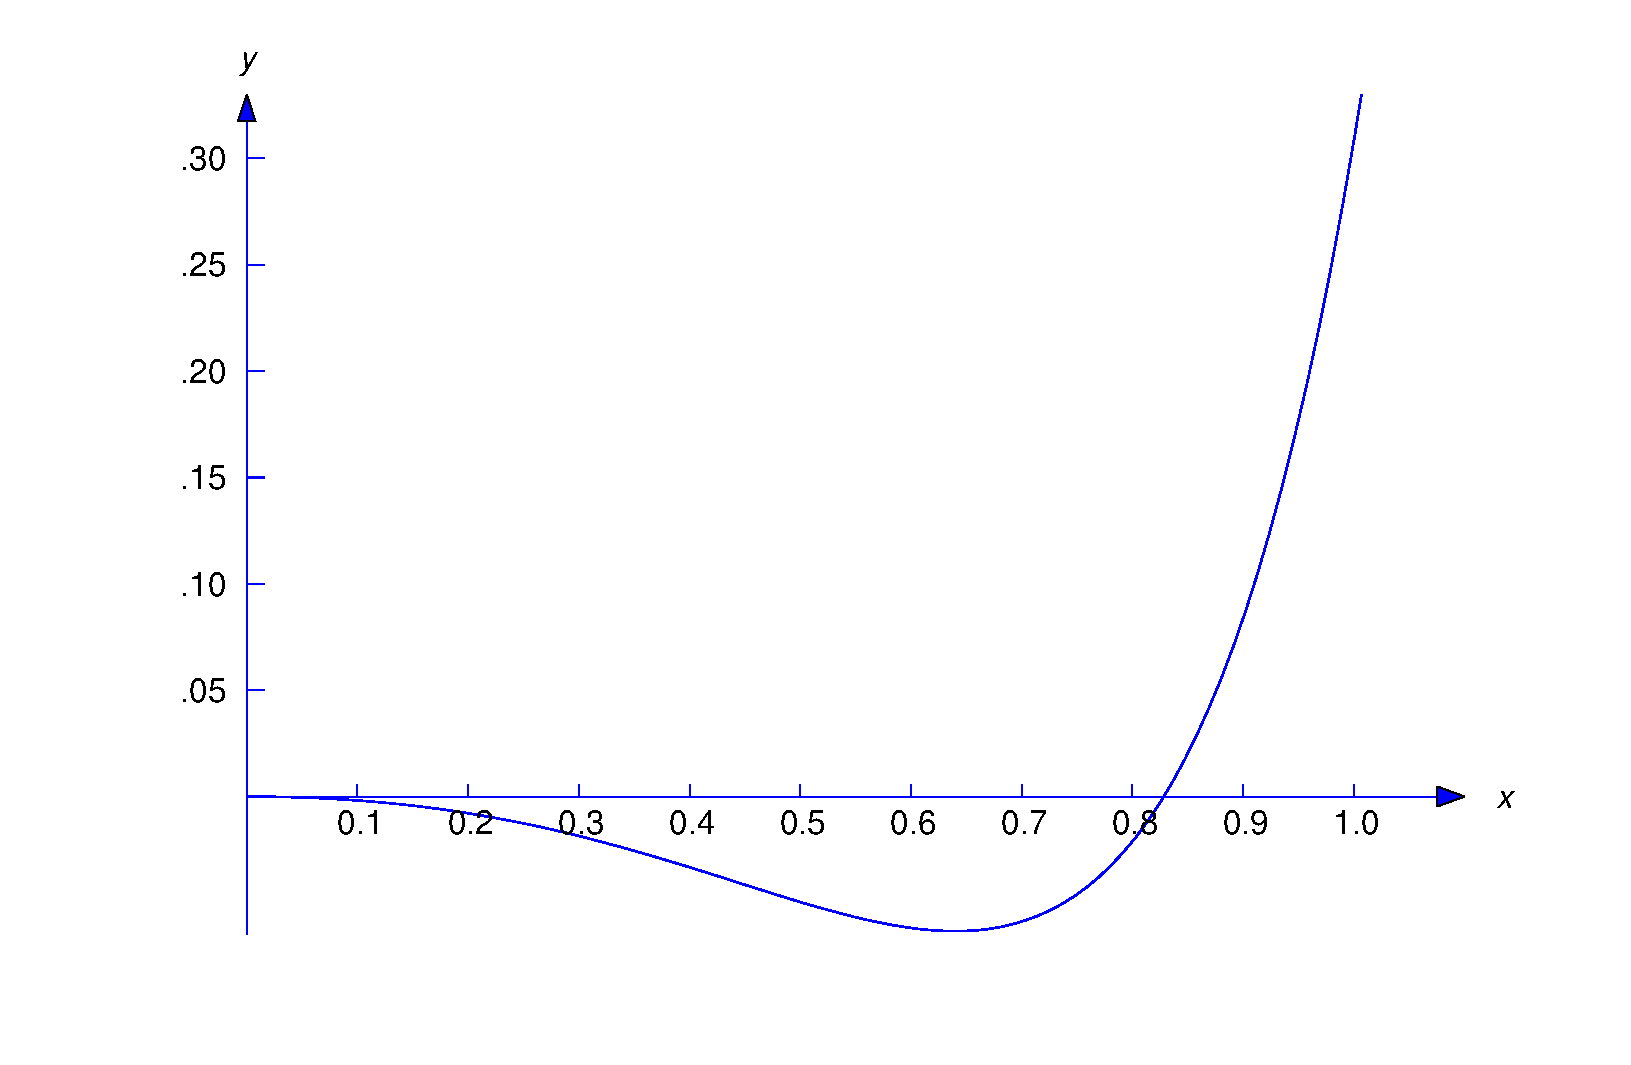
\includegraphics[bb=-78 148 689 643, width=5.67in, height=3.66in, keepaspectratio]{fig090302}
  \caption{$y_{p}=\dst{\frac{x^{2}e^{2x}}{24}(-4+4x+x^{2})}$}
  \label{figure:9.3.2}
\end{figure}

\boxit{Forcing Functions of the Form $e^{\lambda x}\left(P(x)\cos\omega x+Q(x)\sin\omega x\right)$}

\noindent
We now consider equations of the form
\[
  a_{0}y^{(n)}+a_{1}y^{(n-1)}+\cdots+a_{n}y= e^{\lambda x}\left(P(x)\cos\omega x+Q(x)\sin\omega x\right),
\]
where $P$ and $Q$ are polynomials.

\begin{example}
  \label{example:9.3.3} \rm Find a particular solution of
  \begin{equation}
    \label{eq:9.3.7}y'''+y''-4y'-4y=e^{x}[(5-5x)\cos x+(2+5x)\sin x].
  \end{equation}
\end{example}

\solution Substituting
\begin{eqnarray*}
  y    & = & ue^{x},           \\
  y'   & = & e^{x}(u'+u),      \\
  y''  & = & e^{x}(u''+2u'+u), \\
  y''' & = & e^{x}(u'''+3u''+3u'+u)
\end{eqnarray*}
into \eqref{eq:9.3.7} and canceling $e^{x}$ yields
\[
  (u'''+3u''+3u'+u)+(u''+2u'+u)-4(u'+u)-4u =(5-5x)\cos x+(2+5x)\sin x,
\]
or
\begin{equation}
  \label{eq:9.3.8}u'''+4u''+u'-6u=(5-5x)\cos x+(2+5x)\sin x.
\end{equation}
Since $\cos x$ and $\sin x$ are not solutions of the complementary equation
\[
  u'''+4u''+u'-6u=0,
\]
a theorem analogous to Theorem~\ref{thmtype:5.5.1} implies that \eqref{eq:9.3.8} has a particular
solution of the form
\begin{equation}
  \label{eq:9.3.9}u_{p}=(A_{0}+A_{1}x)\cos x+(B_{0}+B_{1}x)\sin x.
\end{equation}
Then
\begin{eqnarray*}
  u_{p}'=(A_{1}+B_{0}+B_{1}x)\cos x+(B_{1}-A_{0}-A_{1}x)\sin x,\\ u_{p}''=(2B_{1}-A_{0}-A_{1}x)\cos x-(2A_{1}+B_{0}+B_{1}x)\sin x,\\ u_{p}'''=-(3A_{1}+B_{0}+B_{1}x)\cos x-(3B_{1}-A_{0}-A_{1}x)\sin x,\\
\end{eqnarray*}
so
\[
  \begin{array}{rcl}
    u_{p}'''+4u_{p}''+u_{p}'-6u_{p} & = & -\left[10A_{0}+2A_{1}-8B_{1}+10A_{1}x\right]\cos x  \\
                                    &   & -\left[10B_{0}+2B_{1}+8A_{1}+10B_{1}x\right]\sin x.
  \end{array}
\]
Comparing the coefficients of $x\cos x$, $x\sin x$, $\cos x$, and $\sin x$ here with the
corresponding coefficients in \eqref{eq:9.3.8} shows that $u_{p}$ is a solution of \eqref{eq:9.3.8}
if
\[
  \begin{array}{rcr}
    -10A_{1}               & = & -5\phantom{.}           \\
    -10B_{1}               & = & \phantom{-}5\phantom{.} \\
    -10A_{0}-2A_{1}+8B_{1} & = & 5\phantom{.}            \\
    -10B_{0}-2B_{1}-8A_{1} & = & 2.
  \end{array}
\]
Solving the first two equations yields $A_{1}=1/2$, $B_{1}=-1/2$. Substituting these into the last
two equations yields
\begin{eqnarray*}
  -10A_{0} & = & 5+2A_{1}-8B_{1}=10\phantom{.} \\
  -10B_{0} & = & 2+2B_{1}+8A_{1}=5,
\end{eqnarray*}
so $A_{0}=-1$, $B_{0}=-1/2$. Substituting $A_{0}=-1$, $A_{1}=1/2$, $B_{0}=-1/2$, $B_{1}=-1/2$ into
\eqref{eq:9.3.9} shows that
\[
  u_{p}=-\dst\frac{1}{2}\left[(2-x)\cos x+(1+x)\sin x\right]
\]
is a particular solution of \eqref{eq:9.3.8}, so
\[
  y_{p}=e^{x}u_{p}=-\frac{e^{x}}{2}\left[(2-x)\cos x+(1+x)\sin x\right]
\]
is a particular solution of \eqref{eq:9.3.7} (Figure~\ref{figure:9.3.3}).

\begin{figure}[tbp]
  \centering
  \color{blue}
  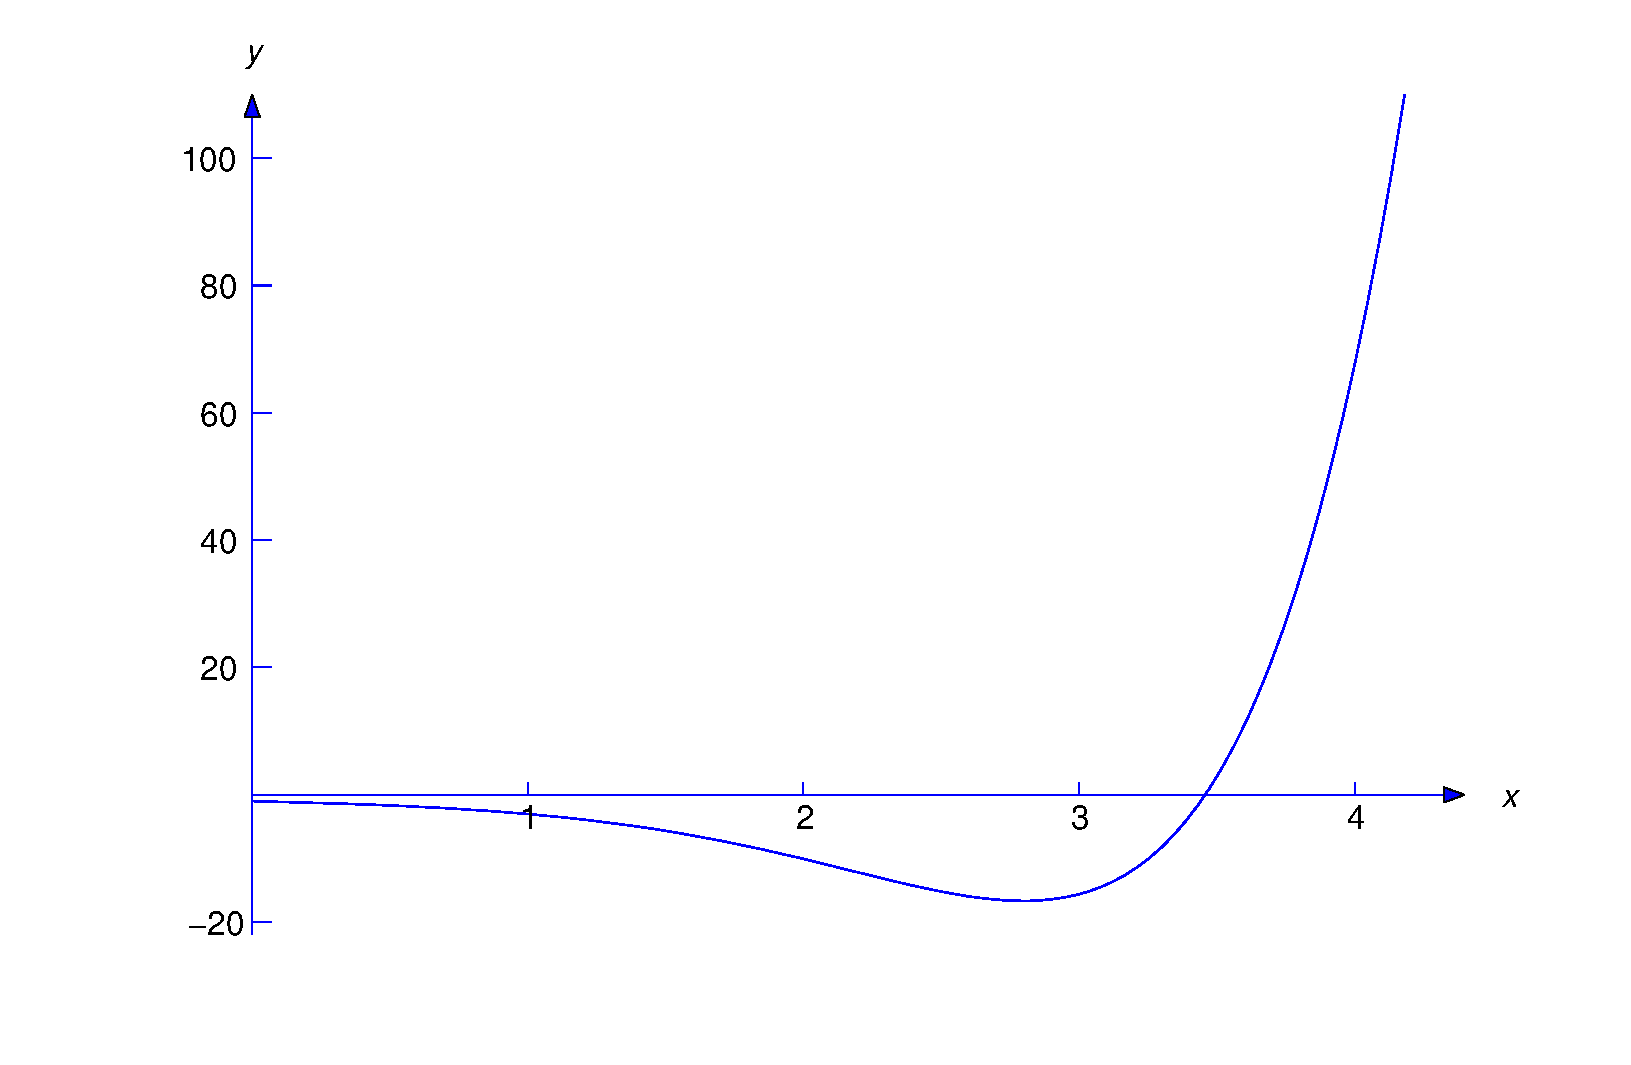
\includegraphics[bb=-78 148 689 643, width=5.67in, height=3.66in, keepaspectratio]{fig090303}
  \caption{$y_{p}=\dst{e^{x}u_{p}=-\frac{e^{x}}{2}\left[(2-x)\cos x+(1+x)\sin x\right]}$}
  \label{figure:9.3.3}
\end{figure}

\begin{example}
  \label{example:9.3.4} \rm Find a particular solution of
  \begin{equation}
    \label{eq:9.3.10}y'''+4y''+6y'+4y= e^{-x}\left[(1-6x)\cos x-(3+2x)\sin x\right].
  \end{equation}
\end{example}

\solution Substituting
\begin{eqnarray*}
  y    & = & ue^{-x},           \\
  y'   & = & e^{-x}(u'-u),      \\
  y''  & = & e^{-x}(u''-2u'+u), \\
  y''' & = & e^{-x}(u'''-3u''+3u'-u)
\end{eqnarray*}
into \eqref{eq:9.3.10} and canceling $e^{-x}$ yields
\[
  (u'''-3u''+3u'-u)+4(u''-2u'+u)+6(u'-u)+4u =(1-6x)\cos x-(3+2x)\sin x,
\]
or
\begin{equation}
  \label{eq:9.3.11}u'''+u''+u'+u=(1-6x)\cos x-(3+2x)\sin x.
\end{equation}
Since $\cos x$ and $\sin x$ are solutions of the complementary equation
\[
  u'''+u''+u'+u=0,
\]
a theorem analogous to Theorem~\ref{thmtype:5.5.1} implies that \eqref{eq:9.3.11} has a particular
solution of the form
\begin{equation}
  \label{eq:9.3.12}u_{p}=(A_{0}x+A_{1}x^{2})\cos x+(B_{0}x+B_{1}x^{2})\sin x.
\end{equation}
\newpage

Then
\begin{eqnarray*}
  u_{p}'   & = & [A_{0}+(2A_{1}+B_{0})x+B_{1}x^{2}]\cos x+[B_{0}+(2B_{1}-A_{0})x-A_{1}x^{2}]\sin x, \\
  u_{p}''  & = & [2A_{1}+2B_{0}-(A_{0}-4B_{1})x-A_{1}x^{2}]\cos x                                   \\
           &   & +[2B_{1}-2A_{0}-(B_{0}+4A_{1})x-B_{1}x^{2}]\sin x,                                 \\
  u_{p}''' & = & -[3A_{0}-6B_{1}+(6A_{1}+B_{0})x+B_{1}x^{2}]\cos x                                  \\
           &   & -[3B_{0}+6A_{1}+(6B_{1}-A_{0})x-A_{1}x^{2}]\sin x,
\end{eqnarray*}
so
\[
  \begin{array}{rcl}
    u_{p}'''+u_{p}''+u_{p}'+u_{p} & = & -[2A_{0}-2B_{0}-2A_{1}-6B_{1}+(4A_{1}-4B_{1})x]\cos x  \\
                                  &   & -[2B_{0}+2A_{0}-2B_{1}+6A_{1}+(4B_{1}+4A_{1})x]\sin x.
  \end{array}
\]
Comparing the coefficients of $x\cos x$, $x\sin x$, $\cos x$, and $\sin x$ here with the
corresponding coefficients in \eqref{eq:9.3.11} shows that $u_{p}$ is a solution of
\eqref{eq:9.3.11} if
\[
  \begin{array}{rcr}
    -4A_{1}+4B_{1}               & = & -6\phantom{.}           \\
    -4A_{1}-4B_{1}               & = & -2\phantom{.}           \\
    -2A_{0}+2B_{0}+2A_{1}+6B_{1} & = & \phantom{-}1\phantom{.} \\
    -2A_{0}-2B_{0}-6A_{1}+2B_{1} & = & -3.
  \end{array}
\]
Solving the first two equations yields $A_{1}=1$, $B_{1}=-1/2$. Substituting these into the last two
equations yields
\begin{eqnarray*}
  -2A_{0}+2B_{0} & = & \phantom{-}1-2A_{1}-6B_{1}=2\phantom{.} \\
  -2A_{0}-2B_{0} & = & -3+6A_{1}-2B_{1}=4,
\end{eqnarray*}

\begin{figure}[H]
  \centering
  \color{blue}
  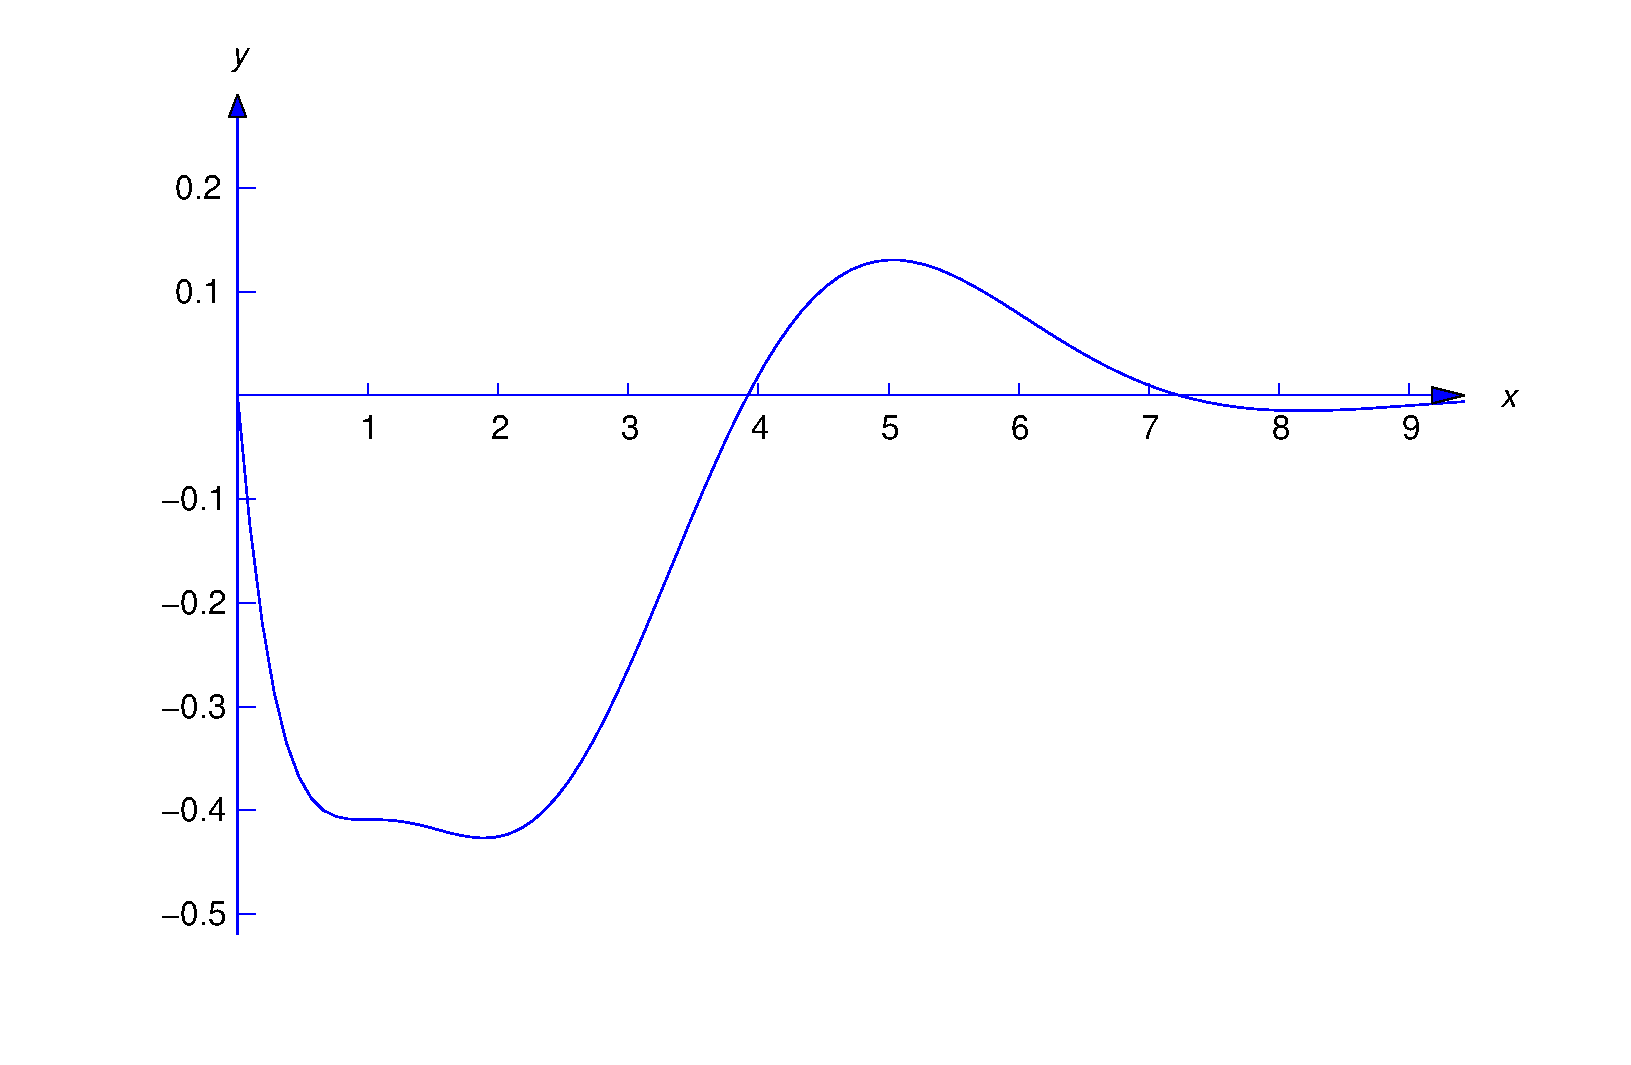
\includegraphics[bb=-78 148 689 643, width=5.67in, height=3.66in, keepaspectratio]{fig090304}
  \caption{$\dst{y_{p}=-\frac{xe^{-x}}{2}\left[(3-2x)\cos x+(1+x)\sin x\right]}$}
  \label{figure:9.3.4}
\end{figure}

\noindent
so $A_{0}=-3/2$ and $B_{0}=-1/2$. Substituting $A_{0}=-3/2$, $A_{1}=1$, $B_{0}=-1/2$, $B_{1}=-1/2$
into \eqref{eq:9.3.12} shows that
\[
  u_{p}=-\dst\frac{x}{2}\left[(3-2x)\cos x+(1+x)\sin x\right]
\]
is a particular solution of \eqref{eq:9.3.11}, so
\[
  y_{p}=e^{-x}u_{p}=-\frac{xe^{-x}}{2}\left[(3-2x)\cos x+(1+x)\sin x\right]
\]
(Figure~\ref{figure:9.3.4}) is a particular solution of \eqref{eq:9.3.10}.

\exercises In Exercises~\ref{exer:9.3.1}--\ref{exer:9.3.59} find a particular solution.

\begin{exerciselist}
  \item\label{exer:9.3.1} $y'''-6y''+11y'-6y=-e^{-x}(4+76x-24x^{2})$

  \item\label{exer:9.3.2} $y'''-2y''-5y'+6y=e^{-3x}(32-23x+6x^{2})$

  \item\label{exer:9.3.3} $4y'''+8y''-y'-2y=-e^{x}(4+45x+9x^{2})$

  \item\label{exer:9.3.4} $y'''+3y''-y'-3y=e^{-2x}(2-17x+3x^{2})$

  \item\label{exer:9.3.5} $y'''+3y''-y'-3y=e^{x}(-1+2x+24x^{2}+16x^{3})$

  \item\label{exer:9.3.6} $y'''+y''-2y=e^{x}(14+34x+15x^{2})$

  \item\label{exer:9.3.7} $4y'''+8y''-y'-2y=-e^{-2x}(1-15x)$

  \item\label{exer:9.3.8} $y'''-y''-y'+y=e^{x}(7+6x)$

  \item\label{exer:9.3.9} $2y'''-7y''+4y'+4y=e^{2x}(17+30x)$

  \item\label{exer:9.3.10} $y'''-5y''+3y'+9y=2e^{3x}(11-24x^{2})$

  \item\label{exer:9.3.11} $y'''-7y''+8y'+16y=2e^{4x}(13+15x)$

  \item\label{exer:9.3.12} $8y'''-12y''+6y'-y=e^{x/2}(1+4x)$

  \item\label{exer:9.3.13} $y^{(4)}+3y'''-3y''-7y'+6y=-e^{-x}(12+8x-8x^{2})$

  \item\label{exer:9.3.14} $y^{(4)}+3y'''+y''-3y'-2y=-3e^{2x}(11+12x)$

  \item\label{exer:9.3.15} $y^{(4)}+8y'''+24y''+32y'=-16e^{-2x}(1+x+x^{2}-x^{3})$

  \item\label{exer:9.3.16} $4y^{(4)}-11y''-9y'-2y=-e^{x}(1-6x)$

  \item\label{exer:9.3.17} $y^{(4)}-2y'''+3y'-y=e^{x}(3+4x+x^{2})$

  \item\label{exer:9.3.18} $y^{(4)}-4y'''+6y''-4y'+2y=e^{2x}(24+x+x^{4})$

  \item\label{exer:9.3.19} $2y^{(4)}+5y'''-5y'-2y=18e^{x}(5+2x)$

  \item\label{exer:9.3.20} $y^{(4)}+y'''-2y''-6y'-4y=-e^{2x}(4+28x+15x^{2})$

  \item\label{exer:9.3.21} $2y^{(4)}+y'''-2y'-y=3e^{-x/2}(1-6x)$

  \item\label{exer:9.3.22} $y^{(4)}-5y''+4y=e^{x}(3+x-3x^{2})$

  \item\label{exer:9.3.23} $y^{(4)}-2y'''-3y''+4y'+4y=e^{2x}(13+33x+18x^{2})$

  \item\label{exer:9.3.24} $y^{(4)}-3y'''+4y'=e^{2x}(15+26x+12x^{2})$

  \item\label{exer:9.3.25} $y^{(4)}-2y'''+2y'-y=e^{x}(1+x)$

  \item\label{exer:9.3.26} $2y^{(4)}-5y'''+3y''+y'-y=e^{x}(11+12x)$

  \item\label{exer:9.3.27} $y^{(4)}+3y'''+3y''+y'=e^{-x}(5-24x+10x^{2})$

  \item\label{exer:9.3.28} $y^{(4)}-7y'''+18y''-20y'+8y=e^{2x}(3-8x-5x^{2})$

  \item\label{exer:9.3.29} $y'''-y''-4y'+4y=e^{-x}\left[(16+10x)\cos x+(30-10x)\sin x\right]$

  \item\label{exer:9.3.30} $y'''+y''-4y'-4y=e^{-x}\left[(1-22x)\cos 2x-(1+6x)\sin2x\right]$

  \item\label{exer:9.3.31} $y'''-y''+2y'-2y=e^{2x}[(27+5x-x^{2})\cos x+(2+13x+9x^{2})\sin x]$

  \item\label{exer:9.3.32} $y'''-2y''+y'-2y=-e^{x}[(9-5x+4x^{2})\cos 2x-(6-5x-3x^{2})\sin2x]$

  \item\label{exer:9.3.33} $y'''+3y''+4y'+12y=8\cos2x-16\sin2x$

  \item\label{exer:9.3.34} $y'''-y''+2y=e^{x}[(20+4x)\cos x-(12+12x)\sin x]$

  \item\label{exer:9.3.35} $y'''-7y''+20y'-24y=-e^{2x}[(13-8x)\cos 2x-(8-4x)\sin2x]$

  \item\label{exer:9.3.36} $y'''-6y''+18y'=-e^{3x}[(2-3x)\cos 3x-(3+3x)\sin3x]$

  \item\label{exer:9.3.37} $y^{(4)}+2y'''-2y''-8y'-8y=e^{x}(8\cos x+16\sin x)$

  \item\label{exer:9.3.38} $y^{(4)}-3y'''+2y''+2y'-4y=e^{x}(2\cos2x -\sin2x)$

  \item\label{exer:9.3.39} $y^{(4)}-8y'''+24y''-32y'+15y=e^{2x}(15x\cos2x+32\sin2x)$

  \item\label{exer:9.3.40} $y^{(4)}+6y'''+13y''+12y'+4y=e^{-x}[(4-x)\cos x-(5+x)\sin x]$

  \item\label{exer:9.3.41} $y^{(4)}+3y'''+2y''-2y'-4y=-e^{-x}(\cos x-\sin x)$

  \item\label{exer:9.3.42} $y^{(4)}-5y'''+13y''-19y'+10y=e^{x}(\cos2x+\sin2x)$

  \item\label{exer:9.3.43} $y^{(4)}+8y'''+32y''+64y'+39y=e^{-2x}[(4-15x)\cos3x-(4+15x)\sin 3x]$

  \item\label{exer:9.3.44} $y^{(4)}-5y'''+13y''-19y'+10y=e^{x}[(7+8x)\cos 2x+(8-4x)\sin2x]$

  \item\label{exer:9.3.45} $y^{(4)}+4y'''+8y''+8y'+4y=-2e^{-x}(\cos x-2\sin x)$

  \item\label{exer:9.3.46} $y^{(4)}-8y'''+32y''-64y'+64y=e^{2x}(\cos2x-\sin2x)$

  \item\label{exer:9.3.47} $y^{(4)}-8y'''+26y''-40y'+25y=e^{2x}[3\cos x-(1+3x)\sin x]$

  \item\label{exer:9.3.48} $y'''-4y''+5y'-2y=e^{2x}-4e^{x}-2\cos x+4\sin x$

  \item\label{exer:9.3.49} $y'''-y''+y'-y=5e^{2x}+2e^{x}-4\cos x+4\sin x$

  \item\label{exer:9.3.50} $y'''-y'=-2(1+x)+4e^{x}-6e^{-x}+96e^{3x}$

  \item\label{exer:9.3.51} $y'''-4y''+9y'-10y=10e^{2x}+20e^{x}\sin2x-10$

  \item\label{exer:9.3.52} $y'''+3y''+3y'+y=12e^{-x}+9\cos2x-13\sin2x$

  \item\label{exer:9.3.53} $y'''+y''-y'-y=4e^{-x}(1-6x)-2x\cos x+2(1+x)\sin x$

  \item\label{exer:9.3.54} $y^{(4)}-5y''+4y=-12e^{x}+6e^{-x}+10\cos x$

  \item\label{exer:9.3.55} $y^{(4)}-4y'''+11y''-14y'+10y=-e^{x}(\sin x+2\cos2x)$

  \item\label{exer:9.3.56} $y^{(4)}+2y'''-3y''-4y'+4y=2e^{x}(1+x)+e^{-2x}$

  \item\label{exer:9.3.57} $y^{(4)}+4y=\sinh x\cos x-\cosh x\sin x$

  \item\label{exer:9.3.58} $y^{(4)}+5y'''+9y''+7y'+2y=e^{-x}(30+24x)-e^{-2x}$

  \item\label{exer:9.3.59} $y^{(4)}-4y'''+7y''-6y'+2y=e^{x}(12x-2\cos x+2\sin x)$

  \exercisetext{In Exercises~\ref{exer:9.3.60}--\ref{exer:9.3.68} find the general solution.}

  \item\label{exer:9.3.60} $y'''-y''-y'+y=e^{2x}(10+3x)$

  \item\label{exer:9.3.61} $y'''+y''-2y=-e^{3x}(9+67x+17x^{2})$

  \item\label{exer:9.3.62} $y'''-6y''+11y'-6y=e^{2x}(5-4x-3x^{2})$

  \item\label{exer:9.3.63} $y'''+2y''+y'=-2e^{-x}(7-18x+6x^{2})$

  \item\label{exer:9.3.64} $y'''-3y''+3y'-y=e^{x}(1+x)$

  \item\label{exer:9.3.65} $y^{(4)}-2y''+y=-e^{-x}(4-9x+3x^{2})$

  \item\label{exer:9.3.66} $y'''+2y''-y'-2y=e^{-2x}\left[(23-2x)\cos x+(8-9x)\sin x\right]$

  \item\label{exer:9.3.67} $y^{(4)}-3y'''+4y''-2y'=e^{x}\left[(28+6x)\cos 2x+(11-12x)\sin2x\right]$

  \item\label{exer:9.3.68} $y^{(4)}-4y'''+14y''-20y'+25y=e^{x}\left[(2+6x)\cos 2x+3\sin2x\right]$

  \exercisetext{In Exercises~\ref{exer:9.3.69}--\ref{exer:9.3.74} solve the initial value problem
  and graph the solution.}

  \item\label{exer:9.3.69}
        \CGex\ $y'''-2y''-5y'+6y=2e^{x}(1-6x),\quad y(0)=2, \quad y'(0)=7,\quad y''(0)=9$

  \item\label{exer:9.3.70}
        \CGex\ $y'''-y''-y'+y=-e^{-x}(4-8x),\quad y(0)=2, \quad y'(0)=0,\quad y''(0)=0$

  \item\label{exer:9.3.71}
        \CGex\ $4y'''-3y'-y=e^{-x/2}(2-3x),\quad y(0)=-1, \quad y'(0)=15,\quad y''(0)=-17$

  \item\label{exer:9.3.72}
        \CGex\ $y^{(4)}+2y'''+2y''+2y'+y=e^{-x}(20-12x),\, y(0)=3,\;y'(0)=-4,\;y''(0)=7,\;y'''(0)=-22$

  \item\label{exer:9.3.73}
        \CGex\ $y'''+2y''+y'+2y=30\cos x-10\sin x, \quad y(0)=3,\quad y'(0)=-4,\quad y''(0)=16$

  \item\label{exer:9.3.74} \CGex\ $y^{(4)}-3y'''+5y''-2y'=-2e^{x}(\cos x-\sin x),\;y(0)=2,\;y'(0)=0,\;y''(0)~=~-1,\\\hspace*{30pt}y'''(0)=-5$

  \item\label{exer:9.3.75} Prove: A function $y$ is a solution of the constant coefficient
        nonhomogeneous equation
  \[
    a_{0}y^{(n)}+a_{1}y^{(n-1)}+\cdots+a_{n}y=e^{\alpha x}G(x) \eqno{\rm(A)}
  \]
  if and only if $y=ue^{\alpha x}$, where $u$ satisfies the differential equation
  \[
    a_{0}u^{(n)}+\frac{p^{(n-1)}(\alpha)}{(n-1)!}u^{(n-1)}+ \frac{p^{(n-2)}(\alpha)}{(n-2)!}u^{(n-2)}+\cdots+p(\alpha)u=G(x) \eqno{\rm(B)}
  \]
  and
  \[
    p(r)=a_{0}r^{n}+a_{1}r^{n-1}+\cdots+a_{n}
  \]
  is the characteristic polynomial of the complementary equation
  \[
    a_{0}y^{(n)}+a_{1}y^{(n-1)}+\cdots+a_{n}y=0.
  \]
  \rm

  \item\label{exer:9.3.76} Prove:
  \begin{alist}
    \item % (a)
    The equation
    \[
      \begin{array}{lcl}
        a_{0}u^{(n)} & + & \dst\frac{p^{(n-1)}(\alpha)}{(n-1)!}u^{(n-1)}+ \dst\frac{p^{(n-2)}(\alpha)}{(n-2)!}u^{(n-2)}+\cdots+p(\alpha)u \\
                     & = & \left(p_{0}+p_{1}x+\cdots+p_{k}x^{k}\right)\cos \omega x                                                       \\
                     &   & \,+\left(q_{0}+q_{1}x+\cdots+q_{k}x^{k}\right)\sin\omega x
      \end{array}
      \eqno{\rm(A)}
    \]
    has a particular solution of the form
    \[
      u_{p}=x^{m}\left(u_{0}+u_{1}x+\cdots+u_{k}x^{k}\right)\cos\omega x+ \left(v_{0}+v_{1}x+\cdots+v_{k}x^{k}\right)\sin\omega x.
    \]

    \item % (b)
    If $\lambda+i\omega$ is a zero of $p$ with multiplicity $m\ge1$, then (A) can be written as
    \[
      a(u''+\omega^{2}u)= \left(p_{0}+p_{1}x+\cdots+p_{k}x^{k}\right)\cos\omega x+ \left(q_{0}+q_{1}x+\cdots+q_{k}x^{k}\right)\sin\omega x,
    \]
    which has a particular solution of the form
    \[
      u_{p}=U(x)\cos\omega x+V(x)\sin\omega x,
    \]
    where
    \[
      U(x)=u_{0}x+u_{1}x^{2}+\cdots+u_{k}x^{k+1},\,V(x)=v_{0}x+v_{1}x^{2}+\cdots+v_{k}x^{k+1}
    \]
    and
    \[
      \begin{array}{rcl}
        a(U''(x)+2\omega V'(x)) & = & p_{0}+p_{1}x+\cdots+p_{k}x^{k}  \\[10pt]
        a(V''(x)-2\omega U'(x)) & = & q_{0}+q_{1}x+\cdots+q_{k}x^{k}.
      \end{array}
    \]
  \end{alist}
  \rm
\end{exerciselist}
